\documentclass[main.tex]{subfiles}
\begin{document}
\section{Secondary Cosmic Rays Detection with Two Geiger-Müller Tubes}
\subsection{Introduction}
The idea to detect cosmic rays by registering simultanous discharges in Geiger-Müller tubes is almost as old as GM tubes themselves. Walther Bothe and Werner Kolhörster published the results from a coincidence experiment with discharges in GM counters in 1929 (“Das Wesen der Höhenstrahlung”, Zeitschrift für Physik 1929,
56: 751), while GM tube was invented in 1928. They registered deflections of fiber electrometers on moving film to detect symyultanous discharges \cite{congresso-nazionale-astronomia2005}.
The first modern, analogous to AND gate, system for detection of symultanous discharges was proposed by Bruno Rossi in 1930 \cite{rossi1930}.

In XIX ceuntry, due to very low prices of electrical components, the experiments which were conducted on the state of art devices in 30's, are possible to repeat in schools' and hobbyists' laboratories. Recently, many experiments detecting muons by the means of two Geiger-Müller tubes were reported on various physical blogs on the Internet and were performed by many students in school laboratories.

The aim of this artcile is to report in possibly rigorous way one of such experiments conducted in hobbiest's laboratory and compare empirical count rate of symultanous discharges in GM tubes with theoretically predicted count rate of muons passing exactly through both GM tubes. We hope that the results could help studends to project their own experiments and to make necessary calculations.   
\subsection{Description of the Experimental Setup}
In the experiment, two electric boards with Geiger-Muller (GM) tubes were fixed to a retord stand in such a way that the tubes were in horisontal position, parallel to each other, one exatly above the other in such a way that the vertical line could be drawn through its centers. The intention of this setup was to register the rate of ``simultaneous'' discharges caused by particles traveling down from the upper parts of the Earth atmosfere. The experiment was performed for (?) various distances of the tubes (...).

 
Equimpent used:
\begin{enumerate}
\item Assembled DIY Geiger-Muller Counter Kit with GM Tube SBM20 with date mark 8903 
\item Assembled DIY Geiger-Muller Counter Kit with GM Tube SBM20 with date mark 8904
\item Microcontroler Atmel ATMega328P embedded in the board Elegoo Uno R3 with 16MHz clock.
\end{enumerate}

Both Geiger-Muller Counter boards were built from the same specification. 3 pins from Geiger-Muller Counter boards were of our particular interest: +5V, GND and INT. On INT pin the special signal is generated whenever there is a discharge in the GM tube. This signal can trigger ATMega328P interruption if INT output from Geiger-Muller Counter board is connected to the interrupt pin (PIN2 or PIN3) of ATMega328P.

Both Geiger-Muller Counter boards were calibarted before experiment to $400\pm 0.8V$  anode-cathode voltage on GM tube. The readings were done by $1M\Omega$ multimeter and the value read was $6.56\pm 0.01V$ with multiplying factor $61$. 

In the experiment, Elegoo Uno R3 was powered by USB cable from PC. Both Geiger-Muller Counter boards were connected through their +5V pin pararelly to the source of +5V from Elegoo Uno R3 board and grounded by their GND pins to Elegoo Uno R3 board GND pin. INT pin from one Geiger-Muller Counter board (which was placed down) was connected to ATMega328P interrupt pin PIN2 and INT pin from the other Geiger-Muller Counter board (which was placed up) was connected to ATMega328P interrupt pin PIN3.

The software on ATMega328P registered signals on PIN2 and PIN3 caused by discharges in GM tubes and fire up interuptions respectively. It sent a signal through USB to PC if both interruptions fired up in less than
\begin{equation}
\Delta t_{th} = 100\pm 4 \mu \text{s}
\end{equation} time interval. Time of arrival of the signal was logged on PC together with time interval between interuptions.

It might have been temppting to use simple AND gate to register symultanous discharges in GM tubes. But even by AND gate will not answer if impulses were really absolutelly symultanous. They always come in certain, however small, intervals and the impulses also last for some time. While the time interval between impulses for AND gate is certainly of order of magnitute shorter than the time interval measured while registering by microcontroller, we had no practical means of quantitive analisys of the former. Thus we decided on the latter, accepting potentially greater, but measurable error.  
  
\subsection{Background readings}
\label{background_readings}
In order to determine background readings, both GM Counter boards were monitored for 55 908 s commenced at 2019-01-10 23:00:01.
\begin{center}

 \begin{tabular}{||c c c||}
 \hline
 & SBM20 (8903) &  SBM20 (8904)\\ 
 \hline\hline
 discharges: & 20531 & 21522\\
 average waiting time: & $2.7232$s & $2.5978$s\\
 std of waiting time: & $2.7537$s & $2.6158$s\\
 est. expect. waiting time ($\beta$): & $2.72\pm 0.06s$ & $2.60 \pm 0.05$s \\
 est. expect. rate ($\lambda$) & $0.367\pm 0.008 \text{s}^{-1}$ & $0.385\pm 0.008 \text{s}^{-1}$ \\
 \hline
\end{tabular}
\end{center}
\subsection{Differentiating discharges in tubes caused by secondary cosmic ray from random nearly simultaneous discharges}

To detect a charged particle flying from the upper parts of Earth atmosfere by registering ``simultaneous'' discharges in both tubes, we need to define what ``simultaneous'' means in our laboratory conditions and prove that we can distiguish them from random nearly simultaneous discharges in tubes. As first test we put one Geiger-Muller Counter board very close ($2.7\pm 0.1$ cm) above the other and log all events in which discharges in both tubes were registered by microcontroler in an interval 
$\Delta t$ where  $\Delta t < \Delta t_{th} = 100\pm 4 \mu s$. The microcontroler with the Arduino libraries we used could measure time in microseconds with a resolution of $4\mu$s.

We observed tubes for 36 627 $s$ starting at 2019-01-12 12:39:29. During this time we registered 801 such events. In the table below we sumarise the distribution of measured time interval $\Delta t$ between discharges in tubes.
\begin{center}
 \begin{tabular}{||c c||} 
 \hline
 $\Delta t [\mu \text{s}]$ & number of events\\ 
 \hline\hline
 12 & 385\\
 16& 128\\ 20& 114\\ 24& 87\\ 28& 45\\ 32& 28\\ 36& 12\\ 40&1\\ 44&1 \\
 $\Delta t > 44$ & 0 \\
 \hline
\end{tabular}
\end{center}
First thing to notice is that the number of events decreases when the length of interval increases, which should have been exactly in an opposit way if nearly simultaneous discharges had happend only by chance. 
The mean value is $m(\Delta t)=17.12 \mu$s and the standard diviation is $\sigma(\Delta t) = 6.38\mu s$. A good candidate for a threshold is $m(\Delta t) + 3\sigma(\Delta t) = 36.3 \mu$s. Keeping in mind that the resolution of the microcontroler is $4\mu$s, the natural choice is $36\mu$s.

Therefore, our definition of ``simultaneous'' will be, if two discharges appear in both tubes in the time interval less or equal 
\begin{equation}
\Delta t_s = 36 \mu \text{s}.
\end{equation}
Considering the error of our microcontroller, we need to remeber that real $\Delta t_s = 36 \pm 4 \mu$s  

We need to keep in mind that based on empirical data in the above table this definition will introduce additional systematic error $\approx 0.25\%$ for measured count rate of simulatnous discharges.

Now, we need to estimate what are the chances of random discharges in both tubes in interval less than $\Delta t_s = 36\mu \pm 4 $s.
To calculate this, we will assume that discharges in tubes are completly random and independent and as such they follow the Poisson process with $\lambda_A = 0.367\pm 0.008 \text{s}^{-1}$ for the tube with date mark 8903 (called further tube A) and $\lambda_B = 0.385\pm 0.008 \text{s}^{-1}$ for tube with date mark 8904 (called further tube B) as established in Subsection \ref{background_readings}. Let $T_A$ and $T_B$ be random variables which denote the waiting times for discharge respectively for tubes A and B.
Now, consider two types of events:
\begin{enumerate}
\item Discharge in tube A followed by discharge in a tube B in an interval equal or less $\Delta t_s$.
\item Discharge in tube B followed by discharge in a tube A in an interval equal or less $\Delta t_s$.
\end{enumerate}
They constitute two independent Poisson processes with rates respectively.
\begin{enumerate}

\item 
\begin{equation}
\lambda^A_{\Delta t_s} = \lambda_A P(T_B \leq \Delta t_s) = \lambda_A(1 - e^{-\lambda_B \Delta t_s}).
\end{equation}

\item 
\begin{equation}
\lambda^B_{\Delta t_s} = \lambda_B P(T_A \leq \Delta t_s) = \lambda_B(1 - e^{-\lambda_A \Delta t_s}). 
\end{equation} 
\end{enumerate}
Now if we conceptually merge events of the above two types in one Poisson process, it will have the following rate
\begin{equation}
\lambda_{\Delta t_s} = \lambda_A P(T_B \leq \Delta t_s) = \lambda_A(1 - e^{-\lambda_B \Delta t_s}) + \lambda_B(1 - e^{-\lambda_A \Delta t_s}).
\end{equation}
For our current values
\begin{equation}
\lambda_{\Delta t_s} = (1.02 \pm 0.16) \cdot 10^{-5} \text{s}^{-1}.
\end{equation}
Thus, expected waiting time for a spontanous ``simultaneous'' discharge (i.e. in interval equal or less $\Delta t_s = 36 \pm 4 \mu $s) is $(1.00\pm 0.16)\cdot 10^5 $s which is more than 23 hours and a half.
This rate of spontanous ``simultaneous'' discharges is quite satisfactory, however we need to keep in mind that $\lambda_{\Delta t_s}$ is our lower bound of an error for any count rate of particles that we will be able to detect in our experiment. Thus we will assume that any conclusions from the experimnent can be drawn only for the rates which are of at least 2 orders of magnitude greater than $\lambda_{\Delta t_s}$.

\subsection{Theoretical prediction of mouns count rate in our experimental setup}
\label{theoretical_muon_count_rate}

We attemped to predict theoretically the count rate of muons passing exactly through both of our GM tubes (more precisely, through the active volumes of the tubes). We used the value of vertical
intensity of muon flux 
\begin{equation}
I_V=(8.4\pm 0.4)\cdot 10^{-3} \text{cm}^2\text{s}^{-1}\text{sr}^{-1}
\end{equation} 
as determined in \cite{dragic2008} and some of our calculation were inspiried by explanations given in \cite{kuo2010}.

The count rate $d\lambda$ of muons coming from an infinitesimal solid angle element $d\Omega$ of celestial sphere at a zenith angle $\theta$ and passing through an infinitesimal element of surfuce with a vector area $\vec{dS}$ is assumed to be equal to 
\begin{equation}
d\lambda = I_V\cos^n\theta (\vec{\eta}\cdot \vec{dS})d\Omega,
\end{equation}
where $\vec{\eta}$ is a unit vector directed from the infinitesimal element of surfuce $\vec{dS}$ to the infinitesimal solid angle element of celestial sphere $d\Omega$, as ilustarted on Figure \ref{fig:muon_flux}. After \cite{dragic2008}, we assumed $n=1.85\pm0.10$.
\begin{figure}[H]

\centering
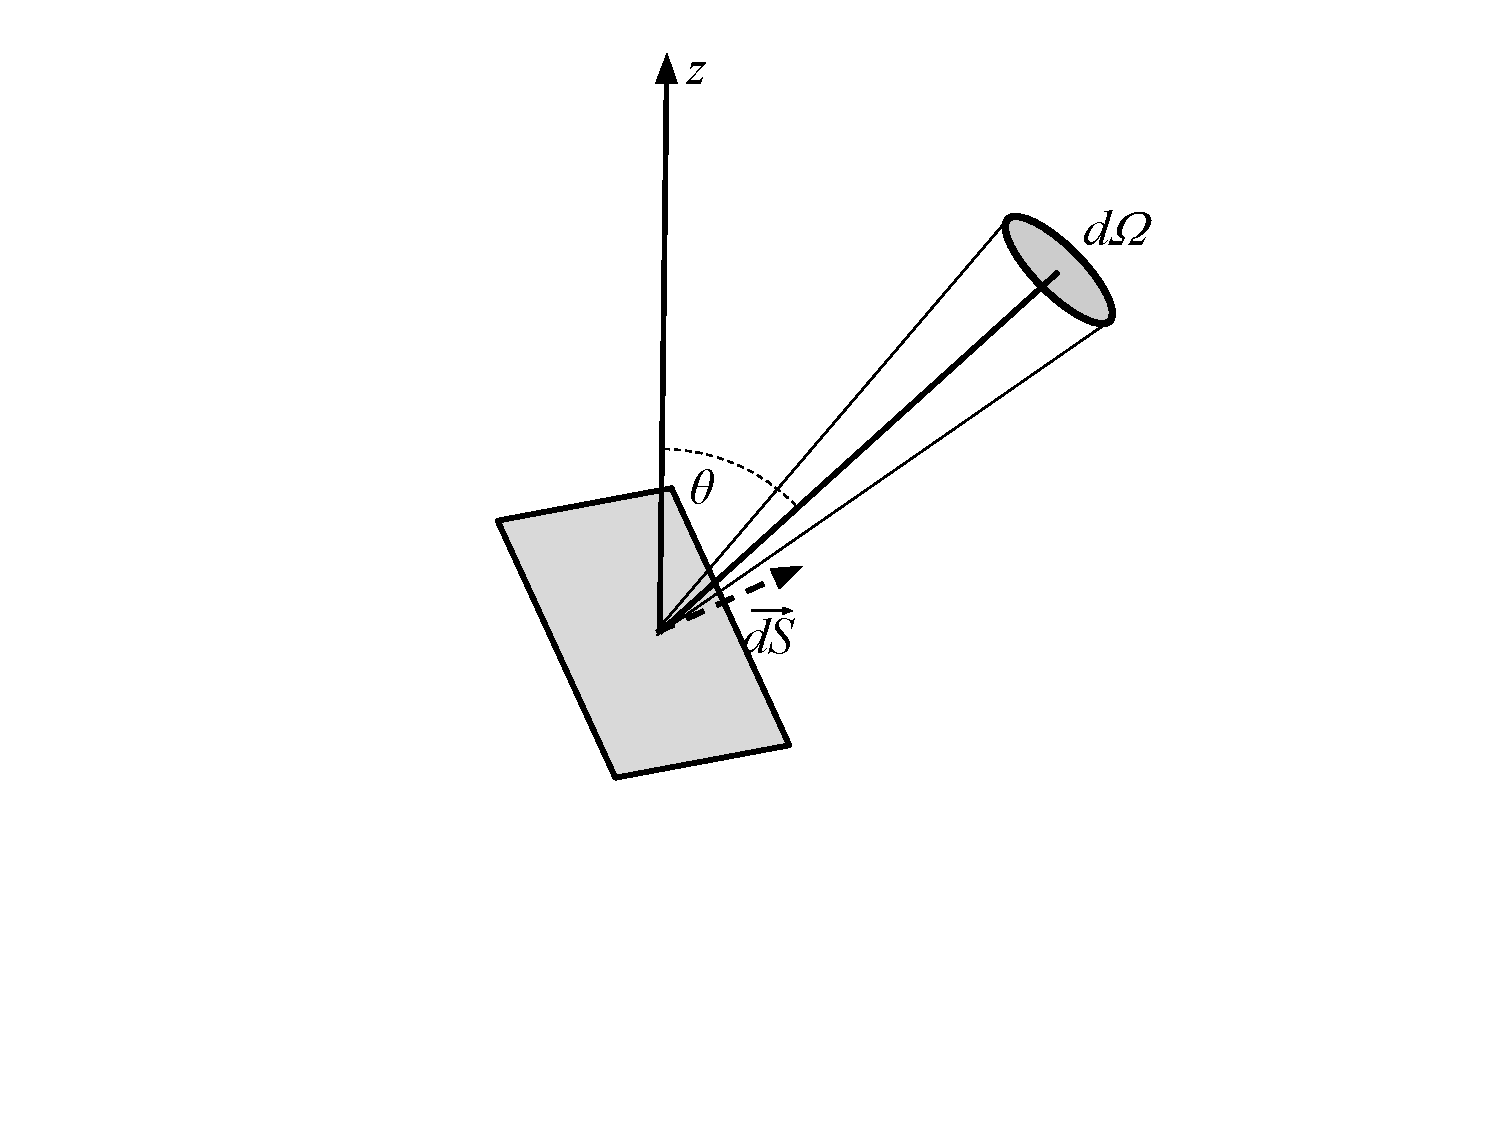
\includegraphics[scale=0.5]{figs/MuonFlux}
\caption{Muon flux through the infinitesimal element of surfuce with a vector area $\vec{dS}$ from an infinitesimal element of celestial sphere with a solid angle $d\Omega$ at a zenith angle $\theta$.}
\label{fig:muon_flux}
\end{figure} 

In case of two cylindrical tubes of the same radious $R$ and of the same length $L$ placed horizontally one above the other in a distance $H$, the total count rate $\lambda$ of muons going exactly through both of the tubes will be given by
\begin{equation}
\label{total-flux-2tubes}
\lambda = I_V\int\limits_{\cup} \int\limits_{\cap}\cos^n\theta (\vec{\eta}\cdot \vec{dS})d\Omega.
\end{equation}
Where an infinitesimal vector area element $\vec{dS}$ runs over the upper part of the lower tube's surface and an infinitesimal solid angle element $d\Omega$ runs over the part of celestial sphere as visible from the point $\vec{dS}$ through the lower half of the upper tube's surface. 

Let's prepare to express an integral \ref{total-flux-2tubes} in variables $x, \alpha$ and $\theta, \phi$ where $x, \alpha$ describe surface coordinates of an element $\vec{dS}$ on the lower tube's surface as in Figure \ref{fig:tubes} and $\theta, \phi$ are respectivelly zenith and azimuth angles of an element $d\Omega$ looking from an element $\vec{dS}$. 

Note that
\begin{equation}
d\Omega = \sin\theta d\theta d\phi.
\end{equation}

We will introduce now help variables $x,z,y$ and $x', z',y'$ in such a way that $(x,z,y)$ are cartesian coordinates of an infinitesimal vector area element $\vec{dS}$ and $(x',z',y')$ are cartesian coordinates of the point where an infinitesimal solid angle element $d\Omega$ crosses the lower half of the upper tube's surface

Note that 
\begin{equation}
\vec{dS} = d\alpha dx R (\cfrac{1}{R}[0,y,z]) = d\alpha dx [0,y,z].
\end{equation}

Now, we can express the integral \ref{total-flux-2tubes} as dependent on $\alpha, x, \theta, \phi$.

\begin{equation}
\label{total-flux-2tubes-2}
\lambda = I_V\int\limits_{\cup} \int\limits_{\cap}\cos^n\theta\sin\theta (\vec{\eta}\cdot [0,y,z]) d\theta d\phi dxd\alpha.
\end{equation}

Next, we prepare to integrate by substitution
\begin{equation}
\label{flux-substitution}
x, \alpha, \theta, \phi \mapsto x,\alpha, x', \alpha'
\end{equation}

where $x', \alpha'$ describe surface coordinates of the point where an infinitesimal solid angle element $d\Omega$ crosses the lower half of the upper tube's surface as in Figure \ref{fig:tubes}.

\begin{figure}[H]
\centering
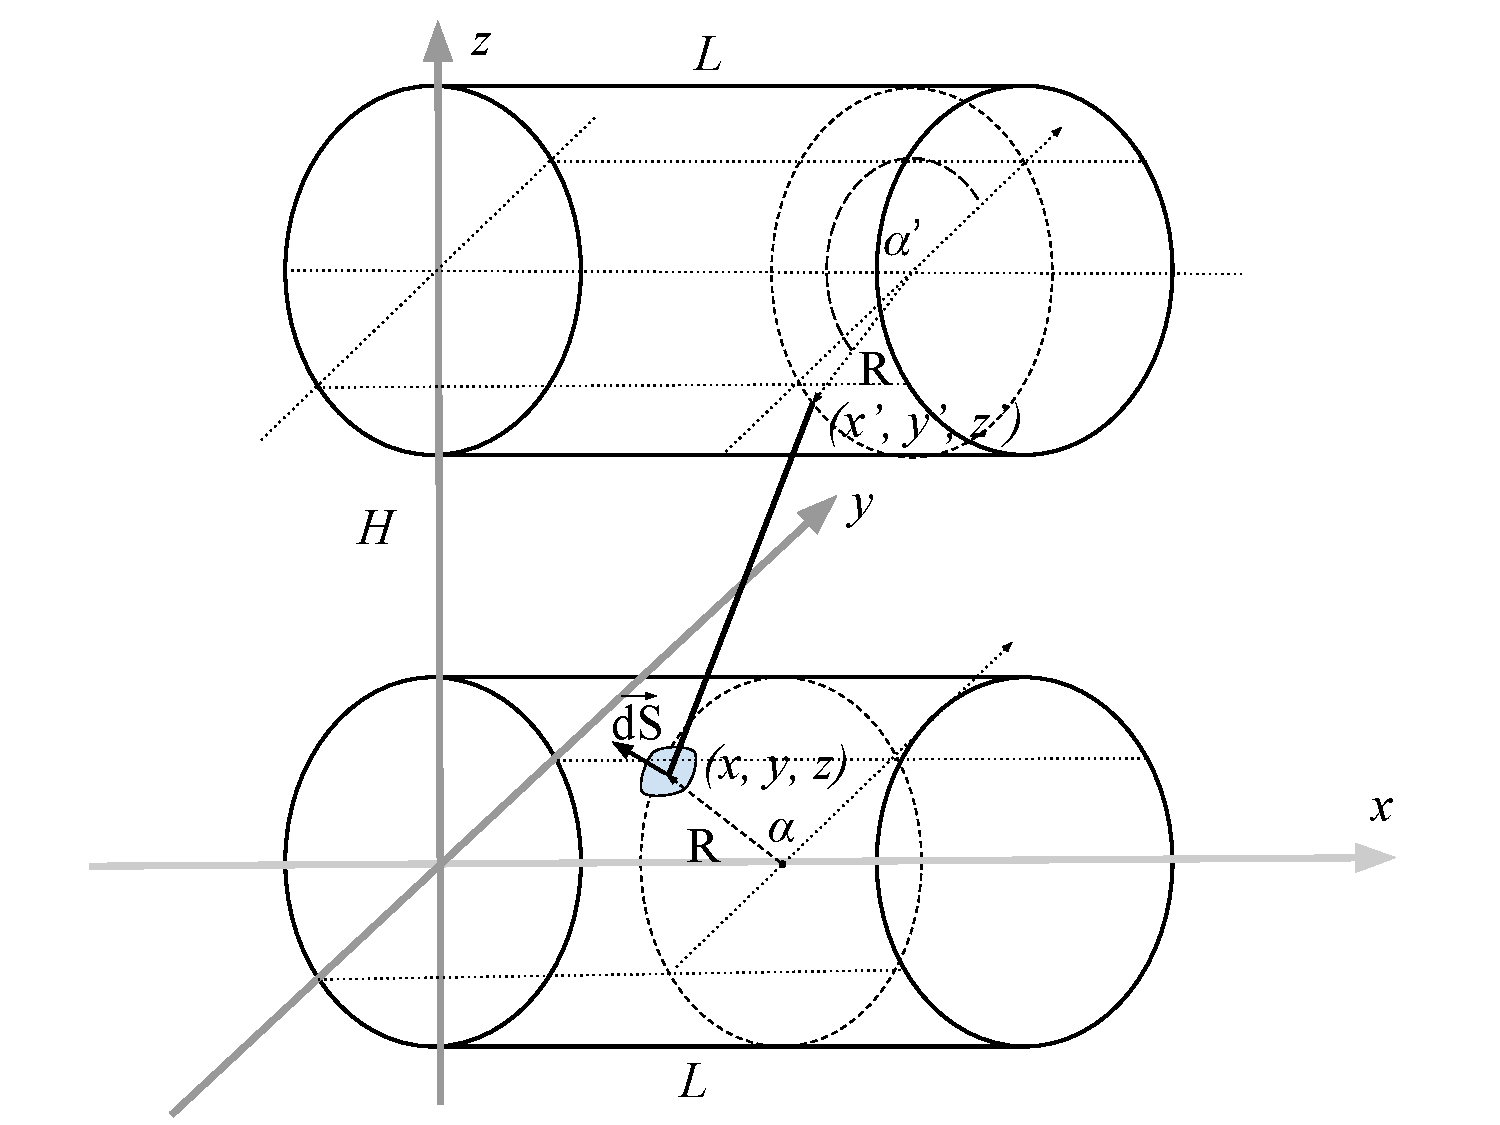
\includegraphics[scale=0.5]{figs/Tubes}
\caption{Muon flux through two GM tubes.}
\label{fig:tubes}
\end{figure}

Let's calculate how $\theta, \phi, \vec{\eta}$ and $y,z$ depends on $x, \alpha, x', \alpha'$. Note that
\begin{equation}
\begin{cases}
y = R \cos\alpha,\\
z = R \sin\alpha\\
y'= R \cos\alpha',\\
z'= R \sin\alpha' + H.\\
\end{cases}
\end{equation}
Now, we can calculate $\theta, \phi, \vec{\eta}$.
\begin{equation}
\begin{cases}
\theta = \arccos(\cfrac{z'-z}{\sqrt{(x'-x)^2 + (y'-y)^2 + (z' - z)^2}}),\\
\phi = \text{arc}((x'- x) +  i(y' - y)),\\
\vec{\eta} = \frac{1}{\sqrt{(x'-x)^2 + (y'-y)^2 + (z' - z)^2}}[x' - x, y' - y, z' - z],\\
\end{cases}
\end{equation}
It is quite obvious that all above variables depend only on $x, \alpha, x', \alpha'$.

To do substitution of variables (\ref{flux-substitution}) in the integral \ref{total-flux-2tubes-2} we need to introduce Jacobian
\begin{equation}
J = 
\begin{bmatrix}
\frac{\partial x}{\partial x} & \frac{\partial x}{\partial \alpha} & \frac{\partial x}{\partial x'} & \frac{\partial x}{\partial \alpha'} \\
\frac{\partial \alpha}{\partial x} & \frac{\partial \alpha}{\partial \alpha} & \frac{\partial \alpha}{\partial x'} & \frac{\partial \alpha}{\partial \alpha'}\\
\frac{\partial \theta}{\partial x} & \frac{\partial \theta}{\partial \alpha} & \frac{\partial \theta}{\partial x'} & \frac{\partial \theta}{\partial \alpha'} \\
\frac{\partial \phi}{\partial x} & \frac{\partial \phi}{\partial \alpha} & \frac{\partial \phi}{\partial x'} & \frac{\partial \phi}{\partial \alpha'} \\
\end{bmatrix}
\end{equation}
After the substitution we have
\begin{equation}
\label{total-flux-2tubes-3}
\lambda = I_V\int\limits_{0}^L\int\limits_{0}^{\pi} \int\limits_{0}^L \int\limits_{\pi}^{2\pi}\cos^n\theta \sin\theta(\vec{\eta}\cdot [0,y,z]) |\det(J)| dxd\alpha dx'd\alpha'.
\end{equation}
We didn't solve the integral (\ref{total-flux-2tubes-3}) manually, instead we used software Mathematica 11 \cite{mathematica2018} to calculate $J$ symbolically and then applied Monte Carlo method (with $5\cdot 10^7$ iterations) for fixed $R, L, H$ to calculate theoretically expected muon count rate $\lambda$ for particular experimental setups.

\subsection{Experimental symultanous discharge count rate v. theoretical muon count rate}

In the table below we will compare theoretical results calculated by integral (\ref{total-flux-2tubes-3}) with experimental count rate of symultanous discharges. For used GM tubes SBM20, we assumed after official specification for active length and active radious
\begin{equation}
\begin{cases}
L = 9.1\pm0.1 \text{cm},\\
R = 1.0\pm0.1 \text{cm}.
\end{cases}
\end{equation}

\begin{tabulary}{\linewidth}{CCCCC}
\hline
 GM tubes distance [cm] & predicted muon count rate [$\text{s}^{-1}$]& observed symult. discharges count rate [$\text{s}^{-1}$]& observation time [s] & observed symult. discharges \\ 
 \hline\hline
 $2.7\pm0.1$ & $0.031\pm0.009$ & $0.022\pm0.002$ & 36 627 & 801\\
 $4.2\pm0.1$ & $0.0185\pm0.0055$ & $0.014\pm0.002$& 43 557 & 611\\
 $7.9\pm0.1$& $(7.9\pm2.1)\cdot 10^{-3}$ & $(5.2\pm0.7)\cdot 10^{-3}$ &106 971&545\\
$11.2\pm0.1$&$(4.7\pm 1.3)\cdot 10^{-3}$&$(3.1\pm 0.4)\cdot 10^{-3}$&141 383&437\\
 \hline
\end{tabulary} 
\end{document}